\begin{frame}
    \frametitle{Analyze for these slides}
    
    \begin{itemize}
    \item EKF-SLAM
    \item Graph-SLAM / Factor Graph
    \item Loop-Closure
    \item Bundle Adjustment
    \end{itemize}
    
    \end{frame}
    
    \begin{frame}
    \frametitle{What is SLAM?}
    
    For a mobile robot to navigate autonomously, it must know its location and have a representation of the environment it is in. These problems are known as the Localization and Mapping problems. In the most general case, where neither the robot's location nor an a priori map of the environment is available, these problems are addressed simultaneously. This gives rise to the SLAM problem (\emph{Simultaneous Localization and Mapping}).
    \begin{block}{}
    SLAM is the problem of solving localization and mapping at the same time.
    \end{block}
    
    \end{frame}
    
    
    \begin{frame}
     \frametitle{SLAM example}
    
     \begin{figure}
     \subfloat[Reality]
     {
     \fbox{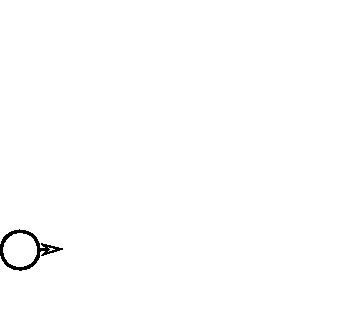
\includegraphics[width=0.44\textwidth]{slam_example_gt1.pdf}}
     }\hfill{}
     \subfloat[Robot SLAM system]
     {
     \fbox{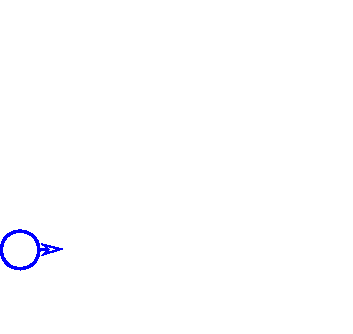
\includegraphics[width=0.44\textwidth]{slam_example_robot1.pdf}}
     }
     \end{figure}
    
    \end{frame}
    
    \begin{frame}
     \frametitle{SLAM example}
     \TODO{improve by making map points adjust too}
     \begin{figure}
     \subfloat[Reality]
     {
     \fbox{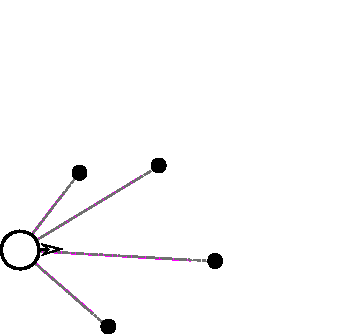
\includegraphics[width=0.44\textwidth]{slam_example_gt2.pdf}}
     }\hfill{}
     \subfloat[Robot SLAM system]
     {
     \fbox{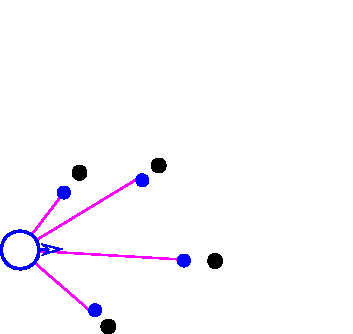
\includegraphics[width=0.44\textwidth]{slam_example_robot2.pdf}}
     }
     \end{figure}
    
    \end{frame}
    
    \begin{frame}
     \frametitle{SLAM example}
    
     \begin{figure}
     \subfloat[Reality]
     {
     \fbox{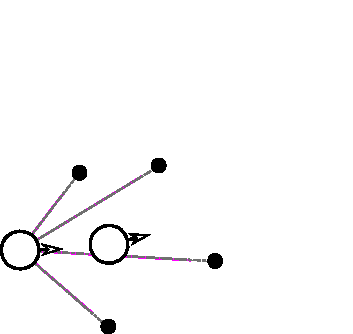
\includegraphics[width=0.44\textwidth]{slam_example_gt3.pdf}}
     }\hfill{}
     \subfloat[Robot SLAM system]
     {
     \fbox{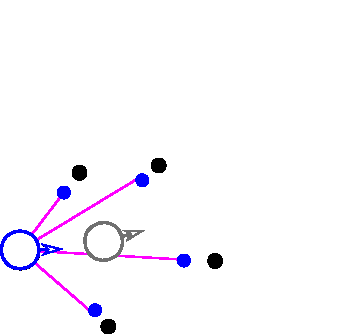
\includegraphics[width=0.44\textwidth]{slam_example_robot3.pdf}}
     }
     \end{figure}
    
    \end{frame}
    
    \begin{frame}
     \frametitle{SLAM example}
    
     \begin{figure}
     \subfloat[Reality]
     {
     \fbox{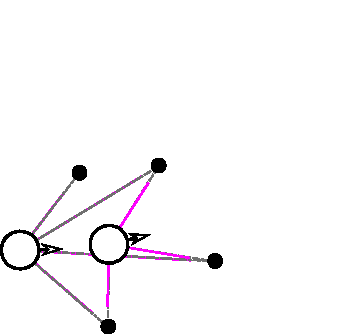
\includegraphics[width=0.44\textwidth]{slam_example_gt4.pdf}}
     }\hfill{}
     \subfloat[Robot SLAM system]
     {
     \fbox{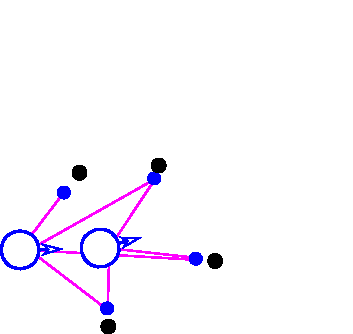
\includegraphics[width=0.44\textwidth]{slam_example_robot4.pdf}}
     }
     \end{figure}
    
    \end{frame}
    
    \begin{frame}
     \frametitle{SLAM example}
    
     \begin{figure}
     \subfloat[Reality]
     {
     \fbox{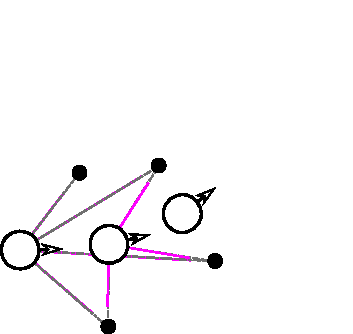
\includegraphics[width=0.44\textwidth]{slam_example_gt5.pdf}}
     }\hfill{}
     \subfloat[Robot SLAM system]
     {
     \fbox{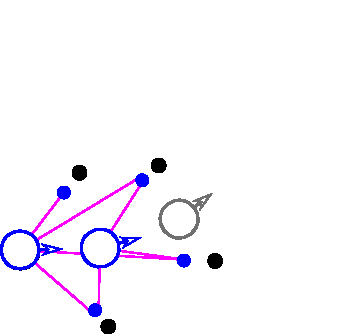
\includegraphics[width=0.44\textwidth]{slam_example_robot5.pdf}}
     }
     \end{figure}
    
    \end{frame}
    
    \begin{frame}
     \frametitle{SLAM example}
    
     \begin{figure}
     \subfloat[Reality]
     {
     \fbox{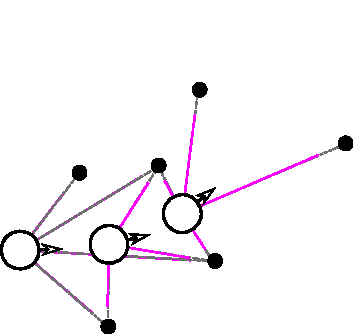
\includegraphics[width=0.44\textwidth]{slam_example_gt6.pdf}}
     }\hfill{}
     \subfloat[Robot SLAM system]
     {
     \fbox{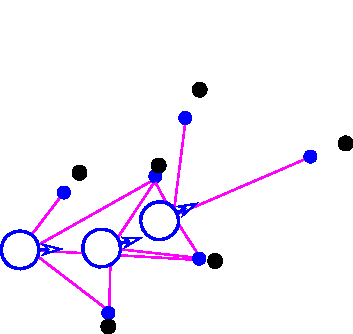
\includegraphics[width=0.44\textwidth]{slam_example_robot6.pdf}}
     }
     \end{figure}
    
    \end{frame}
    
    \begin{frame}
     \frametitle{SLAM example}
    
     \begin{figure}
     \subfloat[Reality]
     {
     \fbox{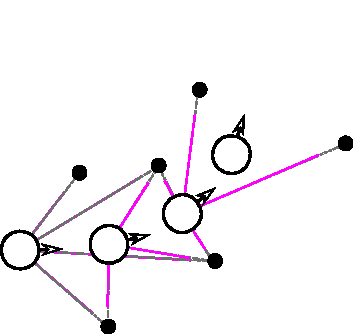
\includegraphics[width=0.44\textwidth]{slam_example_gt7.pdf}}
     }\hfill{}
     \subfloat[Robot SLAM system]
     {
     \fbox{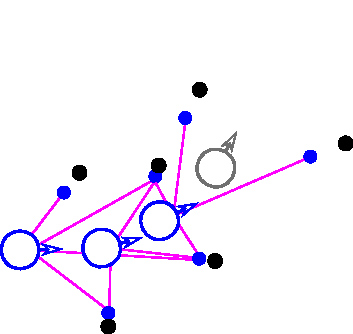
\includegraphics[width=0.44\textwidth]{slam_example_robot7.pdf}}
     }
     \end{figure}
    
    \end{frame}
    
    \begin{frame}
     \frametitle{SLAM example}
    
     \begin{figure}
     \subfloat[Reality]
     {
     \fbox{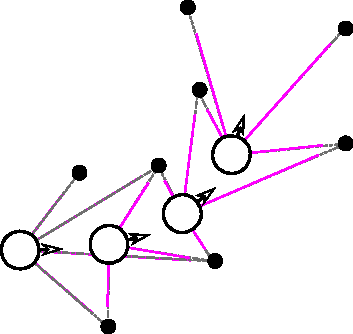
\includegraphics[width=0.44\textwidth]{slam_example_gt8.pdf}}
     }\hfill{}
     \subfloat[Robot SLAM system]
     {
     \fbox{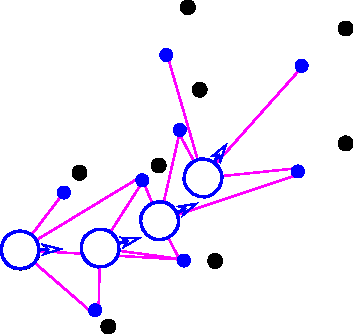
\includegraphics[width=0.44\textwidth]{slam_example_robot8.pdf}}
     }
     \end{figure}
    
    \end{frame}
    
    \begin{frame}
     \frametitle{General SLAM architecture}
    
     \begin{figure}[!h]
     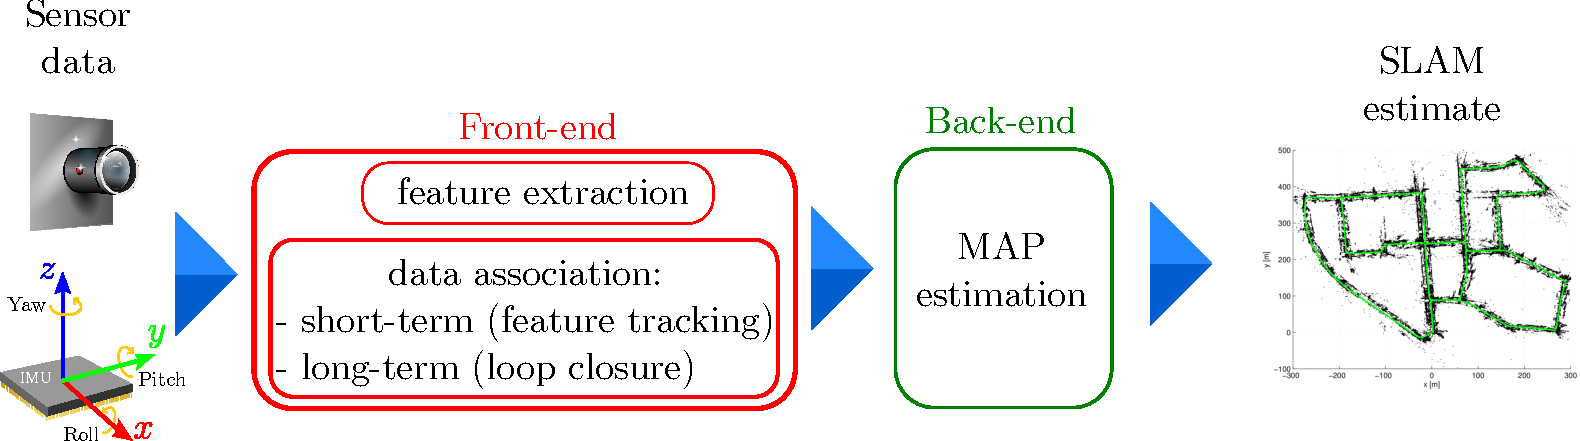
\includegraphics[width=\textwidth]{images/slam_frontend_backend.pdf}
     \end{figure}
    
\end{frame}

\begin{frame}
    \frametitle{Types of SLAM Back-ends}
    \note{Information taken from https://youtu.be/BuRCJ2fegcc and https://youtu.be/Alu59K8zvYs}
    \footnotesize
    \begin{itemize}
    \item Based on Kalman Filter (EKF-SLAM)
    \item Based on Particle Filter (FastSLAM, Rao-Blackwellized Particle Filter, Gmapping)
    \item Based on Least-Squares (Graph-SLAM, Bundle Adjustment)
    \begin{itemize}
    \item Pose-Graph (only contains the robot poses; the map is marginalized.\footnote{Marginalization is the process of removing variables without losing information.})
    \item Factor-Graph (contains poses and landmarks)
    \end{itemize}
    Optimization Tools
    \begin{itemize}
    \item Ceres
    \item GTSAM
    \item g2o
    \end{itemize}
    \end{itemize}
    
    \begin{center}
    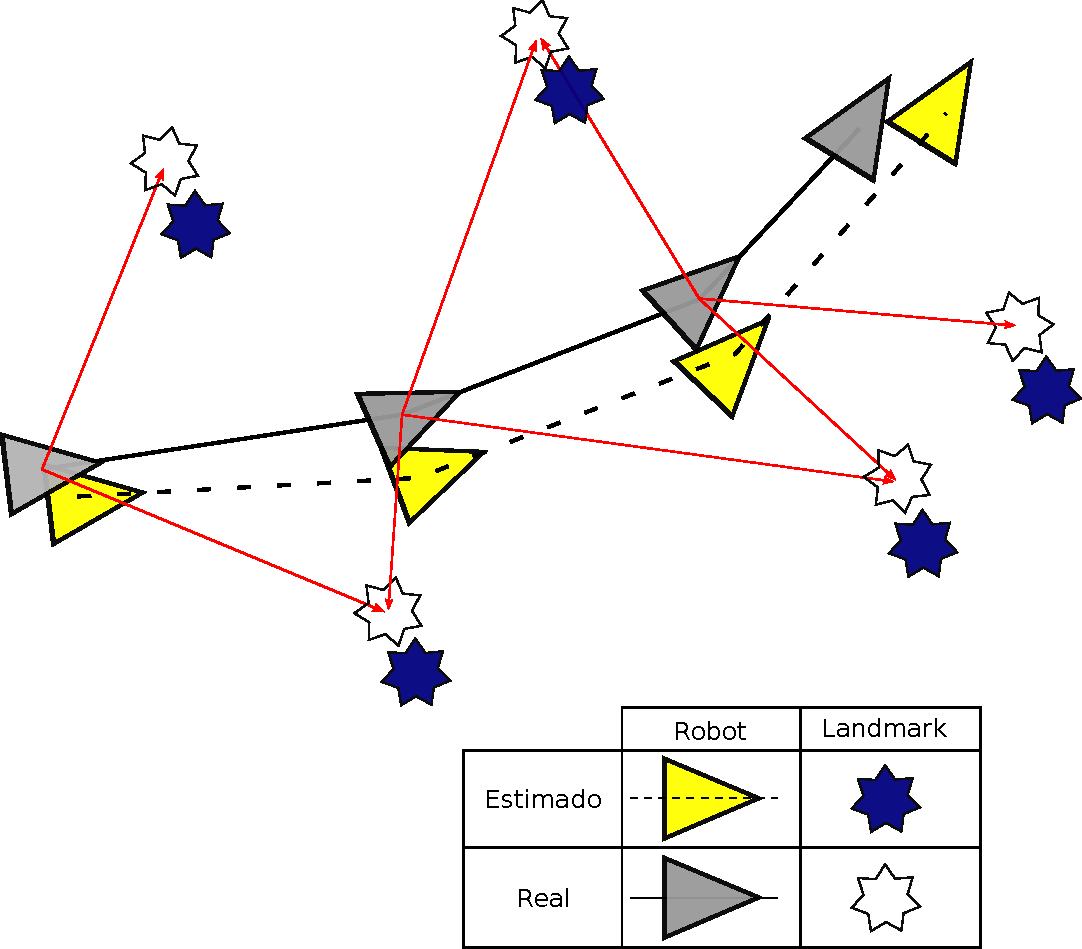
\includegraphics[width=0.25\textwidth]{images/slam-landmarks.pdf}
    \end{center}
    
    \end{frame}
    
    